\chapter{}
\label{lecture11}
%Мы начинаем основную часть курса --- раздел <<уравнения математической физики>>. В этой части мы изучим, во-первых, уравнения, описывающие колебания распределённых систем, во-вторых, уравнения, описывающие распространение тепла в распределённых системах, а также основные методы решения этих --- и не только этих --- уравнений.

\section{Уравнение малых колебаний струны.}
\label{lecture11section1}

\begin{Def}
	Струна --- это гибкая тонкая нить, не сопротивляющаяся изгибу. Внутренние силы возникают в ней только за счёт растяжения.
\end{Def}
Пусть струна в положении равновесия занимает отрезок $[a,b]$ оси $x$, а отклонение точки $x$ в момент $t$ есть $\bm{u}(x,t)$. Для простоты будем считать, что отклонения всех точек $x$ перпендикулярны к отрезку $[a,b]$ и лежат в одной плоскости --- плоскости чертежа и поэтому далее $\bm{u}(x,t)\rightarrow u(x,t)$.

\begin{figure}[H]\centering
\tikzset{every picture/.style={line width=0.75pt}} %set default line width to 0.75pt        

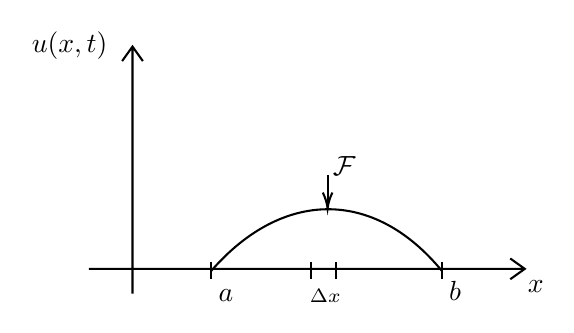
\begin{tikzpicture}[x=0.75pt,y=0.75pt,yscale=-1,xscale=1]
	%uncomment if require: \path (0,162); %set diagram left start at 0, and has height of 162
	
	%Shape: Axis 2D [id:dp3248327615291966] 
	\draw  (37,131.1) -- (247,131.1)(58,24) -- (58,143) (240,126.1) -- (247,131.1) -- (240,136.1) (53,31) -- (58,24) -- (63,31)  ;
	%Straight Lines [id:da25556170305382886] 
	\draw    (96,136) -- (96,128) ;
	%Straight Lines [id:da25576160043853746] 
	\draw    (207,136) -- (207,128) ;
	%Curve Lines [id:da4799623928387329] 
	\draw    (96,132) .. controls (130,93) and (174,92) .. (207,132) ;
	%Straight Lines [id:da6286410245396021] 
	\draw    (152,86) -- (152,100) ;
	\draw [shift={(152,102)}, rotate = 270] [color={rgb, 255:red, 0; green, 0; blue, 0 }  ][line width=0.75]    (7.65,-2.3) .. controls (4.86,-0.97) and (2.31,-0.21) .. (0,0) .. controls (2.31,0.21) and (4.86,0.98) .. (7.65,2.3)   ;
	%Straight Lines [id:da026907285186595242] 
	\draw    (144,136) -- (144,128) ;
	%Straight Lines [id:da12754670649056732] 
	\draw    (156,136) -- (156,128) ;
	
	% Text Node
	\draw (98,139.4) node [anchor=north west][inner sep=0.75pt]    {$a$};
	% Text Node
	\draw (209,135.4) node [anchor=north west][inner sep=0.75pt]    {$b$};
	% Text Node
	\draw (153,75.4) node [anchor=north west][inner sep=0.75pt]    {$\mathcal{F}$};
	% Text Node
	\draw (142,139.4) node [anchor=north west][inner sep=0.75pt]  [font=\scriptsize]  {$\Delta x$};
	% Text Node
	\draw (247,135.4) node [anchor=north west][inner sep=0.75pt]    {$x$};
	% Text Node
	\draw (8,15.4) node [anchor=north west][inner sep=0.75pt]    {$u( x,t)$};
	
	
\end{tikzpicture}
\caption{~}
\label{l11:fig:1}
\end{figure}
Чтобы описать колебания струны, то есть движение её точек под действием внутренних и внешних потенциальных сил воспользуемся принципом Гамильтона. Составим интеграл энергии
\begin{equation*}
	\J[u]=\int\limits_{t_0}^{t_1}\big[T(t)-V(t)\big]\,dt,
\end{equation*}
где $T$ и $V$ --- кинетическая и потенциальная энергии струны. Найдём первую вариацию $\delta\J$ и затем из равенства $\delta\J=0$ получим уравнение колебаний струны и --- в соответствующих случаях --- граничные условия как ЕГУ (естественные граничные условия).

Пусть струна оттянута от положения равновесия и отпущена. Мы рассматриваем только малые колебания: $|u_x(x,t)|\ll1$.

\noindent\parbox{\textwidth}{\centering Энергия струны:}
\begin{gather*}
	\text{кинетическая}\rightarrow T=T_{\text{р}}+T_{\text{с}},\quad V=V_{\text{р}}+V_{\text{с}}\leftarrow\text{потенциальная},
\end{gather*}

\noindent где <<р>> и <<с>> означают соответственно энергию распределённой системы и энергию, связанную с сосредоточенным источником. Найдём выражения для $T_{\text{р}},\ T_{\text{с}},\ V_{\text{р}},\ V_{\text{с}}$ начиная с $T_{\text{р}}$. Кинетическая энергия $\Delta T$ элементарного участка $\Delta x$ есть
\begin{equation*}
	\Delta T_{\text{р}}=\Delta m\cdot\frac{u^2_t(x,t)}{2}=\rho\cdot\Delta x\cdot \frac{u^2_t(x,t)}{2},
\end{equation*}  	   
где $\Delta m$ --- масса участка $\Delta x$, $\rho$ --- плотность струны. Очевидно, что 
\begin{equation*}
	 T_{\text{р}}=\int\limits_a^{b}\frac{\rho\cdot u^2_t}{2}\,dx.
\end{equation*}

Энергия $T_{\text{с}}$ присутствует, если струна была нагружена одной или несколькими точечными массами. Предположим, что в точке $\overline{x}$ струна нагружена массой $\overline{m}$. Тогда 
\begin{equation*}
	 T_{\text{с}}=\frac{\overline{m}\cdot u^2_t(\overline{x},t)}{2}.
\end{equation*}

Переходим к нахождению потенциальной энергии. В общем случае $V_{\text{р}}=V_{\text{р}_1}+V_{\text{р}_2}$, где $V_{\text{р}_1}$ --- потенциальная энергия струны за счёт её растяжения, а $V_{\text{р}_2}$ --- за счёт работы внешних распределённых сил. Начнём сначала с $V_{\text{р}_1}$. Можно доказать (см. например,~\cite{TihonovSamarskii}), что при малых колебаниях натяжение струны $\mu$ не зависит от удлинения. Поэтому запасённая потенциальная энергия $\Delta V_{\text{р}_1}$ элементарного участка $\Delta x$ пропорциональна его удлинению
\begin{equation*}
	\Delta V_{\text{р}_1}=\mu\cdot\Delta l=\mu\cdot\left(\sqrt{1+u^2_x}\cdot\Delta x-\Delta x\right)\approx\frac{\mu\cdot u^2_x}{2}\cdot\Delta x.\footnotemark{} 
\end{equation*}
\footnotetext{Здесь мы воспользовались приближённой формулой $\sqrt{1+\alpha}\approx 1+\frac{\alpha}{2}$, при $|\alpha|\ll1$.}Следовательно
\begin{equation*}
	 V_{\text{р}_1}=\int\limits_a^b\frac{\mu\cdot u^2_x}{2}\,dx.
\end{equation*}

Найдём $V_{\text{р}_2}$. Пусть на струну действует распределённая сила $\mc{F}$ направленная перпендикулярно к $[a,b]$ в плоскости чертежа и пусть $f(x,t)$~--- линейная плотность этой силы, то есть $f(x,t)$ есть сила, действующая на единицу длины. Сила, действующая на элементарный участок $\Delta x$ --- $\Delta\mc{F}=f\cdot\Delta x$ и поэтому её потенциал $\Delta U=-f(x,t)\cdot\Delta x\cdot u(x,t)$. Следовательно, потенциальная энергия участка $\Delta x$ за счёт силы $\mc{F}$ есть $\Delta V_{\text{р}_2}=\Delta U=-f\cdot u\cdot\Delta x$, а полная потенциальная энергия за счёт действия силы $\mc{F}$ очевидно
\begin{equation*}
	 V_{\text{р}_2}=-\int\limits_a^b f\cdot u\,dx.\footnotemark{}
\end{equation*}
\footnotetext{Здесь мы воспользовались известным из курсов физики фактом, что когда внешняя сила действует на объект, то изменение потенциальной энергии объекта равно потенциалу силы.}

Обсудим теперь величину $V_{\text{с}}$. Предположим, что в точке $\widehat{x}$ на струну действует сосредоточенная сила, перпендикулярная отрезку $[a,b]$ или же (или одновременно) в этой точке к струне прикреплена пружина, которую струна сжимает или растягивает при колебаниях.
\begin{figure}[H]\centering
\tikzset{every picture/.style={line width=0.75pt}} %set default line width to 0.75pt        

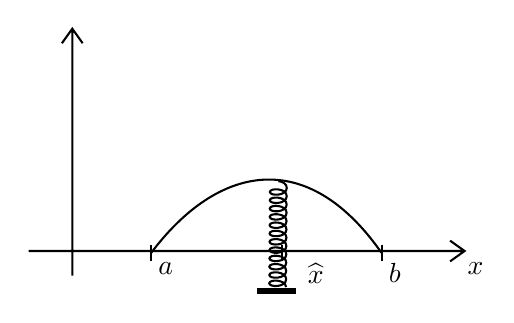
\begin{tikzpicture}[x=0.75pt,y=0.75pt,yscale=-1,xscale=1]
	%uncomment if require: \path (0,162); %set diagram left start at 0, and has height of 162
	
	%Shape: Axis 2D [id:dp568415431333978] 
	\draw  (37,131.1) -- (247,131.1)(58,24) -- (58,143) (240,126.1) -- (247,131.1) -- (240,136.1) (53,31) -- (58,24) -- (63,31)  ;
	%Straight Lines [id:da6315311561256083] 
	\draw    (96,136) -- (96,128) ;
	%Straight Lines [id:da07005979202360346] 
	\draw    (207,136) -- (207,128) ;
	%Curve Lines [id:da644520411610563] 
	\draw    (96,132) .. controls (128,89.5) and (171,80.5) .. (207,132) ;
	%Straight Lines [id:da660057766915144] 
	\draw    (159,136) -- (159,128) ;
	%Shape: Spring [id:dp1849279727639963] 
	\draw   (157.29,97.43) .. controls (159.32,97.69) and (161.35,98.7) .. (161.33,100.7) .. controls (161.31,104.7) and (153.18,104.65) .. (153.19,102.65) .. controls (153.21,100.65) and (161.33,100.7) .. (161.31,104.7) .. controls (161.28,108.7) and (153.15,108.65) .. (153.17,106.65) .. controls (153.18,104.65) and (161.31,104.7) .. (161.28,108.7) .. controls (161.25,112.7) and (153.12,112.65) .. (153.14,110.65) .. controls (153.15,108.65) and (161.28,108.7) .. (161.25,112.7) .. controls (161.22,116.7) and (153.1,116.65) .. (153.11,114.65) .. controls (153.12,112.65) and (161.25,112.7) .. (161.22,116.7) .. controls (161.19,120.7) and (153.07,120.65) .. (153.08,118.65) .. controls (153.1,116.65) and (161.22,116.7) .. (161.19,120.7) .. controls (161.17,124.7) and (153.04,124.65) .. (153.05,122.65) .. controls (153.07,120.65) and (161.19,120.7) .. (161.17,124.7) .. controls (161.14,128.7) and (153.01,128.65) .. (153.03,126.65) .. controls (153.04,124.65) and (161.17,124.7) .. (161.14,128.7) .. controls (161.11,132.7) and (152.99,132.65) .. (153,130.65) .. controls (153.01,128.65) and (161.14,128.7) .. (161.11,132.7) .. controls (161.08,136.7) and (152.96,136.65) .. (152.97,134.65) .. controls (152.99,132.65) and (161.11,132.7) .. (161.08,136.7) .. controls (161.05,140.7) and (152.93,140.65) .. (152.94,138.65) .. controls (152.96,136.65) and (161.08,136.7) .. (161.05,140.7) .. controls (161.03,144.7) and (152.9,144.65) .. (152.92,142.65) .. controls (152.93,140.65) and (161.05,140.7) .. (161.03,144.7) .. controls (161,148.7) and (152.87,148.65) .. (152.89,146.65) .. controls (152.9,144.68) and (160.75,144.7) .. (160.99,148.5) ;
	%Straight Lines [id:da04984138320568832] 
	\draw [line width=2.25]    (147,150.5) -- (166,150.5) ;
	
	% Text Node
	\draw (98,135.4) node [anchor=north west][inner sep=0.75pt]    {$a$};
	% Text Node
	\draw (209,135.4) node [anchor=north west][inner sep=0.75pt]    {$b$};
	% Text Node
	\draw (247,135.4) node [anchor=north west][inner sep=0.75pt]    {$x$};
	% Text Node
	\draw (170,135.4) node [anchor=north west][inner sep=0.75pt]    {$\widehat{x}$};
	
	
\end{tikzpicture}
\caption{~}
\label{l11:fig:2}
\end{figure}

Обозначим изменение энергии струны в точке $\widehat{x}$ через $g$. Выражение для $g$ будет дано позже, а пока только для упрощения дальнейших выкладок предположим, что $\widehat{x}=\overline{x}$. Таким образом
\begin{equation*}
	 V_{\text{с}}=g(t,u(\overline{x},t)).
\end{equation*}

Собирая вместе все составляющие кинетической и потенциальной энергии струны, мы получим интеграл действия в виде
\begin{multline*}
	 \J[u]=\int\limits_{t_0}^{t_1}\!\!\int\limits_a^b\underbrace{\left(\frac{\rho\cdot u^2_t}{2}-\frac{\mu\cdot u^2_x}{2}+f\cdot u\right)}_{F}\,dxdt+\\+\int\limits_{t_0}^{t_1}\underbrace{\left(\frac{\overline{m}\cdot u^2_t(\overline{x},t)}{2}-g(t,u(\overline{x},t))\right)}_{\Phi}\,dt.
\end{multline*}
Обозначим подынтегральное выражение двукратного интеграла через $F=F(x,t,u,u_x,u_t)$, а однократного через $\Phi=\Phi(t,u(\overline{x},t),u_t(\overline{x},t))$ и введём на плоскости $x,t$ область 
\begin{equation*}
	\Omega=\left\{x,t\middle|\, x\in[a,b],\, t\in[t_0,t_1]\right\}.
\end{equation*}
\begin{figure}[H]\centering
\tikzset{every picture/.style={line width=0.75pt}} %set default line width to 0.75pt        

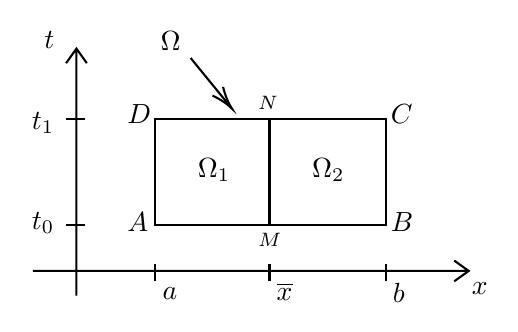
\begin{tikzpicture}[x=0.75pt,y=0.75pt,yscale=-1,xscale=1]
	%uncomment if require: \path (0,162); %set diagram left start at 0, and has height of 162
	
	%Shape: Axis 2D [id:dp033385002892103444] 
	\draw  (37,131.1) -- (247,131.1)(58,24) -- (58,143) (240,126.1) -- (247,131.1) -- (240,136.1) (53,31) -- (58,24) -- (63,31)  ;
	%Straight Lines [id:da23290127141076722] 
	\draw    (96,136) -- (96,128) ;
	%Straight Lines [id:da9776319010753525] 
	\draw    (207,136) -- (207,128) ;
	%Straight Lines [id:da06420289301641557] 
	\draw    (151,136) -- (151,128) ;
	%Shape: Rectangle [id:dp34760015951663625] 
	\draw   (96,58) -- (207,58) -- (207,109) -- (96,109) -- cycle ;
	%Straight Lines [id:da011040244644266117] 
	\draw    (53,109) -- (62,109) ;
	%Straight Lines [id:da4964088587876916] 
	\draw    (53,58) -- (62,58) ;
	%Straight Lines [id:da2828961469522162] 
	\draw    (113,28.5) -- (131.74,51.45) ;
	\draw [shift={(133,53)}, rotate = 230.77] [color={rgb, 255:red, 0; green, 0; blue, 0 }  ][line width=0.75]    (10.93,-3.29) .. controls (6.95,-1.4) and (3.31,-0.3) .. (0,0) .. controls (3.31,0.3) and (6.95,1.4) .. (10.93,3.29)   ;
	%Straight Lines [id:da2101032473064448] 
	\draw    (151,57.5) -- (151,109) ;
	
	% Text Node
	\draw (98,137.4) node [anchor=north west][inner sep=0.75pt]    {$a$};
	% Text Node
	\draw (209,135.4) node [anchor=north west][inner sep=0.75pt]    {$b$};
	% Text Node
	\draw (247,135.4) node [anchor=north west][inner sep=0.75pt]    {$x$};
	% Text Node
	\draw (41,14.4) node [anchor=north west][inner sep=0.75pt]    {$t$};
	% Text Node
	\draw (153,135.4) node [anchor=north west][inner sep=0.75pt]    {$\overline{x}$};
	% Text Node
	\draw (35,101.4) node [anchor=north west][inner sep=0.75pt]    {$t_{0}$};
	% Text Node
	\draw (35,53.4) node [anchor=north west][inner sep=0.75pt]    {$t_{1}$};
	% Text Node
	\draw (81,101.4) node [anchor=north west][inner sep=0.75pt]    {$A$};
	% Text Node
	\draw (81,49.4) node [anchor=north west][inner sep=0.75pt]    {$D$};
	% Text Node
	\draw (208,101.4) node [anchor=north west][inner sep=0.75pt]    {$B$};
	% Text Node
	\draw (208,49.4) node [anchor=north west][inner sep=0.75pt]    {$C$};
	% Text Node
	\draw (97,14.4) node [anchor=north west][inner sep=0.75pt]    {$\Omega $};
	% Text Node
	\draw (144,111.4) node [anchor=north west][inner sep=0.75pt]  [font=\scriptsize]  {$M$};
	% Text Node
	\draw (144,45.4) node [anchor=north west][inner sep=0.75pt]  [font=\scriptsize]  {$N$};
	% Text Node
	\draw (115,75.4) node [anchor=north west][inner sep=0.75pt]    {$\Omega _{1}$};
	% Text Node
	\draw (170,75.4) node [anchor=north west][inner sep=0.75pt]    {$\Omega _{2}$};
	
	
\end{tikzpicture}
\caption{~}
\label{l11:fig:3}
\end{figure}
\noindent Тогда
\begin{equation*}
	\J[u]=\iint\limits_{\Omega}F\,dxdt+\int\limits_{M}^{N}\Phi\,dt\text{, где }M=(\overline{x},t_0),\ N=(\overline{x},t_1).
\end{equation*}

Чтобы найти вариацию от интеграла действия, то есть величину
\begin{equation*}
	\gamma\cdot\left.\der{}{\gamma}\J[u+\gamma\cdot\eta]\right|_{\gamma=0}
\end{equation*}
надо в первую очередь ввести допустимое изменение $\eta(x,t)$ и описать его свойства исходя из того, что функция $u(x,t)+\gamma\cdot\eta(x,t)$ ($\gamma$ --- малый параметр) должна описывать траекторию движения струны из того же начального состояния в то же конечное, что и $u(x,t)$. Так как состояние струны определяется положением каждой точки, то мы потребуем, чтобы  
\begin{equation*}
	 \eta(x,t_0)=\eta(x,t_1)\equiv0,\quad\forall x\in[a,b].
\end{equation*}

Далее при нахождении первой вариации двукратных интегралов в <<Лекциях по вариационному исчислению>>~\cite{VI} мы применяли формулу Остроградского--Гаусса к вектору вида $\bm{W}=\big(F_{u_x}\cdot\eta,F_{u_t}\cdot\eta\big)$\footnote{Там производная была не по $t$, а по $y$, но это не существенно.}. Но применение данной формулы возможно лишь при определённой гладкости компонент этого вектора, а в рассматриваемой ситуации функция $u_x(x,t)$, а следовательно и компоненты вектора $\bm{W}$ могут иметь разрыв при $x=\overline{x}$. Поэтому при нахождении первой вариации интеграла действия мы разобьём область $\Omega$ на две области
\begin{equation*}
	\Omega_{1}=\left\{x,t\middle|\,x\in[a,\overline{x}],\ t\in[t_0,t_1]\right\},\quad	\Omega_{2}=\left\{x,t\middle|\,x\in(\overline{x},b],\ t\in[t_0,t_1]\right\}
\end{equation*} 
и будем брать вариацию по каждой из областей. Имеем 
\begin{equation*}
	\J[u]=\iint\limits_{\Omega_1}F\,dxdt+\iint\limits_{\Omega_2}F\,dxdt+\int\limits_{M}^{N}\Phi\,dt.
\end{equation*}
Предположим, что $a<\overline{x}<b$ и что концы струны или закреплены $u(a,t)=u(b,t)=0$, или движутся по заданным законам $u(a,t)=\nu_1(t)$, $u(b,t)=\nu_2(t)$. В обоих случаях мы должны потребовать, чтобы 
\begin{equation*}
	\eta(a,t)=\eta(b,t)\equiv0,\quad\forall t.
\end{equation*}
Если же $\overline{x}=a\,\{b\}$, то области $\Omega_{1}\,\{\Omega_{2}\}$ не будет, и тогда требование $\eta(a,t)\equiv0\,\{\eta(b,t)\equiv0\}$ отпадает, так как тогда $u(a,t)$ $\{u(b,t)\}$ не задаётся. 

Положим
\begin{gather*}
	\J_j[u]=\iint\limits_{\Omega_j}F(x,t,u,u_x,u_t)\,dxdt,\ j=1,2;\\\J_3[u]=\int\limits_{t_0}^{t_1}\Phi(t,u(\overline{x},t),u_t(\overline{x},t))\,dt.
	\intertext{Тогда}
	\J[u]=\J_1[u]+\J_2[u]+\J_3[u]
	\intertext{и}
	\delta\J=\gamma\cdot\left.\der{}{\gamma}\left\{\sum\limits_{j=1}^2\J_{j}[u+\gamma\cdot\eta]+\J_3[u+\gamma\cdot\eta(\overline{x},t)]\right\}\right|_{\gamma=0}.
\end{gather*}
Используя известные нам формулы первой вариации для двукратных и однократных интегралов получим
\begin{multline*}
	\delta\J=\gamma\cdot\left[\vphantom{\iint\limits_{\Omega_j}}\right.\sum\limits_{j=1}^2\left\{\iint\limits_{\Omega_j}\left(F_{u}-\der{}{x}F_{u_x}-\der{}{t}F_{u_t}\right)\cdot\eta\,dxdt+\right.\\
\end{multline*}
\begin{multline}
	\label{l11:eq:1}
	\hfil\left.\vphantom{\iint\limits_{\Omega_j}}+\int\limits_{\partial\Omega_j}\left(F_{u_x}\cdot\cos\alpha+F_{u_t}\cdot\cos\beta\right)\cdot\eta\,dl\right\}+\\
	\int\limits_{t_0}^{t_1}\left(\Phi_{u}-\der{}{t}\Phi_{u_t}\right)\cdot\eta(\overline{x},t)\,dt+\Phi_{u_t}\cdot\eta(\overline{x},t)\mathop{\Big|}\limits_{t_0}^{t_1}\left.\vphantom{\iint\limits_{\Omega_j}}\right].
\end{multline}
Здесь $\cos\alpha$, $\cos\beta$ --- компоненты единичной внешней нормали к границе области $\Omega_j$ на плоскости $x,t$.
\begin{figure}[H]\centering
\tikzset{every picture/.style={line width=0.75pt}} %set default line width to 0.75pt        

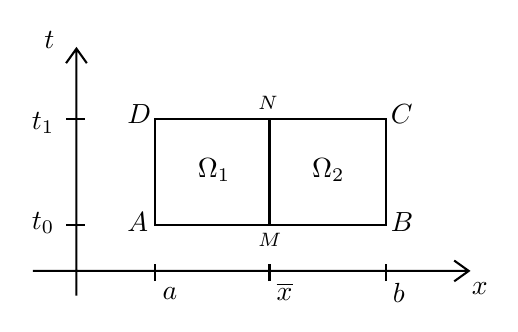
\begin{tikzpicture}[x=0.75pt,y=0.75pt,yscale=-1,xscale=1]
	%uncomment if require: \path (0,162); %set diagram left start at 0, and has height of 162
	
	%Shape: Axis 2D [id:dp2237198969795473] 
	\draw  (37,131.1) -- (247,131.1)(58,24) -- (58,143) (240,126.1) -- (247,131.1) -- (240,136.1) (53,31) -- (58,24) -- (63,31)  ;
	%Straight Lines [id:da4988233348557616] 
	\draw    (96,136) -- (96,128) ;
	%Straight Lines [id:da3469178817338765] 
	\draw    (207,136) -- (207,128) ;
	%Straight Lines [id:da48617665238907604] 
	\draw    (151,136) -- (151,128) ;
	%Shape: Rectangle [id:dp8926884831137676] 
	\draw   (96,58) -- (207,58) -- (207,109) -- (96,109) -- cycle ;
	%Straight Lines [id:da23169370164602432] 
	\draw    (53,109) -- (62,109) ;
	%Straight Lines [id:da7909330230568588] 
	\draw    (53,58) -- (62,58) ;
	%Straight Lines [id:da17521553787578226] 
	\draw    (151,57.5) -- (151,109) ;
	
	% Text Node
	\draw (98,137.4) node [anchor=north west][inner sep=0.75pt]    {$a$};
	% Text Node
	\draw (209,135.4) node [anchor=north west][inner sep=0.75pt]    {$b$};
	% Text Node
	\draw (247,135.4) node [anchor=north west][inner sep=0.75pt]    {$x$};
	% Text Node
	\draw (41,14.4) node [anchor=north west][inner sep=0.75pt]    {$t$};
	% Text Node
	\draw (153,135.4) node [anchor=north west][inner sep=0.75pt]    {$\overline{x}$};
	% Text Node
	\draw (35,101.4) node [anchor=north west][inner sep=0.75pt]    {$t_{0}$};
	% Text Node
	\draw (35,53.4) node [anchor=north west][inner sep=0.75pt]    {$t_{1}$};
	% Text Node
	\draw (81,101.4) node [anchor=north west][inner sep=0.75pt]    {$A$};
	% Text Node
	\draw (81,49.4) node [anchor=north west][inner sep=0.75pt]    {$D$};
	% Text Node
	\draw (208,101.4) node [anchor=north west][inner sep=0.75pt]    {$B$};
	% Text Node
	\draw (208,49.4) node [anchor=north west][inner sep=0.75pt]    {$C$};
	% Text Node
	\draw (144,111.4) node [anchor=north west][inner sep=0.75pt]  [font=\scriptsize]  {$M$};
	% Text Node
	\draw (144,45.4) node [anchor=north west][inner sep=0.75pt]  [font=\scriptsize]  {$N$};
	% Text Node
	\draw (115,75.4) node [anchor=north west][inner sep=0.75pt]    {$\Omega _{1}$};
	% Text Node
	\draw (170,75.4) node [anchor=north west][inner sep=0.75pt]    {$\Omega _{2}$};
	
	
\end{tikzpicture}
\caption{~}
\label{l11:fig:4}
\end{figure}

Так как $\eta(x,t_0)=\eta(x,t_1)=0\,\forall x$, то интегралы по границам областей $\Omega_j$ сведутся к интегралам по $M\!N$ и $D\!A$ для $\Omega_1$ и по $BC$ и $N\!M$ для $\Omega_2$\footnote{Напомним, что положительное направление обхода границы --- обход против часовой стрелки.}. Очевидно, что на отрезках $BC$, $M\!N$, $N\!M$, $D\!A$ выполняется $\cos\beta=0$, так как нормали к ним перпендикулярны к оси $t$. Далее $\cos\alpha=1$ на $BC$ и $M\!N$ и $\cos\alpha=-1$ на $D\!A$ и $N\!M$.

Учитывая вышесказанное и полагая для краткости
\begin{equation*}
	P\eqdef\big(F_{u_x}\cdot\cos\alpha+F_{u_t}\cdot\cos\beta\big)\cdot\eta,
\end{equation*}
имеем
\begin{multline}\label{l11:eq:2}
	\int\limits_{\partial\Omega_1}P\,dl=\int\limits_{t_0}^{t_1}P\bigg|_{\lefteqn{\scriptstyle x=\overline{x}-0}}\,dt\quad+\int\limits_{t_1}^{t_0}P\bigg|_{\lefteqn{\scriptstyle x=a+0}}\,dl\quad=\int\limits_{t_0}^{t_1}P\bigg|_{\lefteqn{\scriptstyle x=\overline{x}-0}}\,dt\quad+\int\limits_{t_0}^{t_1}P\bigg|_{\lefteqn{\scriptstyle x=a+0}}\,dt\quad=\\
	=\int\limits_{t_0}^{t_1}\left[\mu\cdot u_x\bigg|_{\lefteqn{\scriptstyle x=a+0}}\cdot\eta(a,t)-\mu\cdot u_x\bigg|_{\lefteqn{\scriptstyle x=\overline{x}-0}}\cdot\eta(\overline{x},t)\right]\,dt.
\end{multline}  
\begin{multline}
	\label{l11:eq:3}
	\int\limits_{\partial\Omega_2}P\,dl=\int\limits_{t_0}^{t_1}P\bigg|_{\lefteqn{\scriptstyle x=b-0}}\,dt\quad+\int\limits_{t_1}^{t_0}P\bigg|_{\lefteqn{\scriptstyle x=\overline{x}+0}}\,dl\quad=\\=\int\limits_{t_0}^{t_1}\left[-\mu\cdot u_x\bigg|_{\lefteqn{\scriptstyle x=b-0}}\cdot\eta(b,t)+\mu\cdot u_x\bigg|_{\lefteqn{\scriptstyle x=\overline{x}+0}}\cdot\eta(\overline{x},t)\right]\,dt.
\end{multline}
Здесь учтено, что $dl=dt$ при интегрировании по $BC$, $M\!N$ и $dl=-dt$ при интегрировании по $N\!M$ и $D\!A$: появившийся минус мы учли, поменяв местами пределы интегрирования в интергалах от $t_1$ до $t_0$.

Перепишем теперь выражение \eqref{l11:eq:1}, подставляя туда $F$ и $\Phi$. Тогда с учётом равенств \eqref{l11:eq:2} и \eqref{l11:eq:3} получим
\begin{multline}
	\label{l11:eq:4}
	\delta\J=\gamma\cdot\left\{\vphantom{\iint\limits_{\Omega_j}}\right.\!\sum\limits_{j=1}^{2}\iint\limits_{\Omega_j}\left[f+\pder{}{x}\big(\mu\cdot u_x\big)-\pder{}{t}\big(\rho\cdot u_t\big)\right]\cdot\eta\,dxdt+\\
	+\int\limits_{t_0}^{t_1}\left[\mu\cdot u_x\cdot\eta\bigg|_{x=a+0}-\mu\cdot u_x\cdot\eta\bigg|_{x=\overline{x}-0}-\mu\cdot u_x\cdot\eta\bigg|_{x=b-0}+\right.\\\left.+\mu\cdot u_x\cdot\eta\bigg|_{x=\overline{x}+0}-\big(\overline{m}\cdot u_{tt}+g_u\big)\cdot\eta\bigg|_{x=\overline{x}}\,\right]\,dt\!\left.\vphantom{\iint\limits_{\Omega_j}}\right\}.
\end{multline}
Взяв $\eta(a,t)=\eta(b,t)=\eta(\overline{x},t)=0$ и затем $\eta(x,t)\equiv0$, при $(x,t)\in\Omega_2$ получим условие $\delta\J=0$ в виде 
\begin{equation*}
	\iint\limits_{\Omega_1}\left[f+\pder{}{x}\big(\mu\cdot u_x\big)-\pder{}{t}\big(\rho\cdot u_t\big)\right]\cdot\eta\,dxdt=0.
\end{equation*}
Отсюда по лемме Лагранжа для функций двух переменных получаем 
\begin{equation}
	\label{l11:eq:5}
	 f+\pder{}{x}\big(\mu\cdot u_x\big)-\pder{}{t}\big(\rho\cdot u_t\big)=0\quad\text{при }(x,t)\in\Omega_1.
\end{equation}
Аналогично полагая $\eta(x,t)\equiv0$ в области $\Omega_1$, убеждаемся в справедливости уравнения~\eqref{l11:eq:5} для $(x,t)\in\Omega_2$, исключая, быть может, отрезок $x=\overline{x}$, $t\in[t_0,t_1]$. Уравнение~\eqref{l11:eq:5} --- это и есть уравнение колебаний струны.

Если $\overline{x}\neq a,b$, то взяв $\eta(a,t)=\eta(b,t)=0$ мы в силу~\eqref{l11:eq:4} с учётом~\eqref{l11:eq:5} получим
\begin{equation*}
	\int\limits_{t_0}^{t_1}\left[\mu\cdot u_x\bigg|_{x=\overline{x}+0}\!\!\!\!\!\!-\mu\cdot u_x\bigg|_{x=\overline{x}-0}\!\!\!\!\!\!-\overline{m}\cdot u_{tt}(\overline{x},t)-g_u\bigg|_{x=\overline{x}}\right]\cdot\eta(\overline{x},t)\,dt=0,\quad\!\!\!\!\forall\eta(\overline{x},t).
\end{equation*}
Отсюда в силу леммы Лагранжа для однократных интегралов получаем условие при $x=\overline{x}$
\begin{equation}
	\label{l11:eq:6}
	 \mu\cdot u_x\bigg|_{x=\overline{x}+0}-\mu\cdot u_x\bigg|_{x=\overline{x}-0}-\big(\overline{m}\cdot u_{tt}+g_u\big)\bigg|_{x=\overline{x}}=0.
\end{equation}
Вид функции $g$ мы обсудим позже, а пока рассмотрим случаи $\overline{x}=a$ и $\overline{x}=b$. Пусть $\overline{x}=a$, тогда области $\Omega_1$ не будет, и~\eqref{l11:eq:6} запишется в виде 
\begin{equation}
	\label{l11:eq:7}
	\mu\cdot u_x\bigg|_{x=a}=\big(\overline{m}\cdot u_{tt}+g_u\big)\bigg|_{x=a},
\end{equation}
при $\overline{x}=b$ нет области $\Omega_2$ и условие~\eqref{l11:eq:6} можно переписать в виде 
\begin{equation}
	\label{l11:eq:8}
	-\mu\cdot u_x\bigg|_{x=b}=\big(\overline{m}\cdot u_{tt}+g_u\big)\bigg|_{x=b}.
\end{equation} 

Найдём теперь вид функции $g(t,u(\overline{x},t))$ для двух наиболее интересных случаев.
\begin{enumerateA}
	\item\label{l11:enum:A} Пусть в точке $\overline{x}$ действует сосредоточенная сила $f_0(t)$. Потенциал $v_0(t)$ этой силы, очевидно, равен --- $f_0(t)\cdot u(\overline{x},t)$ и, следовательно, $g=v_0=-f_0(t)\cdot u(\overline{x},t)$. В этом случае $g_u=-f_0(t)$ и тогда при $\overline{m}=0$ условие~\eqref{l11:eq:6} перепишется в виде% 
	\addtocounter{equation}{-2}%
	\begin{equation}
		\label{l11:eq:6A}
		\mu\cdot u_x\bigg|_{\overline{x}+0}-\mu\cdot u_x\bigg|_{\overline{x}-0}=-f_0(t), \tag{\theequation{}A}
	\end{equation} 
	а условия \eqref{l11:eq:7} и \eqref{l11:eq:8} в виде%
	\addtocounter{equation}{1}% 
	\begin{equation}
		\label{l11:eq:7A}
		\mu\cdot u_x\bigg|_{x=a}=-f_1(t),\tag{\theequation{}A}
	\end{equation}
	\addtocounter{equation}{1}%
	\begin{equation}
		\label{l11:eq:8A}
		\mu\cdot u_x\bigg|_{x=b}=f_2(t),\tag{\theequation{}A}
	\end{equation}
	где $f_1(t)$ и $f_2(t)$ --- сосредоточенные силы, действующие на концах струны. 
	
	\noindent Если $f_1(t)=f_2(t)\equiv0$, то мы получим условия на свободных концах
	\begin{equation}
		\label{l11:eq:9}
		 \mu\cdot u_x\bigg|_{x=a}=0,\quad\mu\cdot u_x\bigg|_{x=b}=0.
	\end{equation}
	Отметим, что условие \eqref{l11:eq:6A} описывает скачок производной $u_x$ в точке $x=\overline{x}$.
	\item Упругое закрепление. Пусть в точке $x=\overline{x}$ к струне прикреплена пружинка, натянутая на вертикальный стержень (без трения) и закреплённая в точке $C$.
	\begin{figure}[H]\centering
	\tikzset{every picture/.style={line width=0.75pt}} %set default line width to 0.75pt        
	
	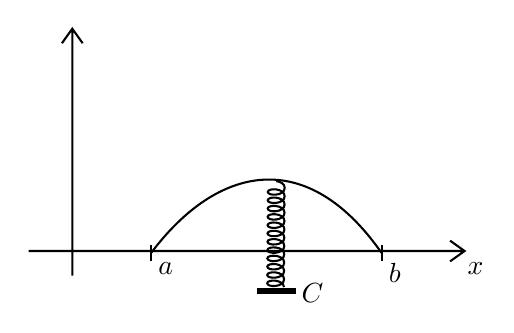
\begin{tikzpicture}[x=0.75pt,y=0.75pt,yscale=-1,xscale=1]
		%uncomment if require: \path (0,162); %set diagram left start at 0, and has height of 162
		
		%Shape: Axis 2D [id:dp3800136695378986] 
		\draw  (37,131.1) -- (247,131.1)(58,24) -- (58,143) (240,126.1) -- (247,131.1) -- (240,136.1) (53,31) -- (58,24) -- (63,31)  ;
		%Straight Lines [id:da6326916483448484] 
		\draw    (96,136) -- (96,128) ;
		%Straight Lines [id:da6653494140567895] 
		\draw    (207,136) -- (207,128) ;
		%Curve Lines [id:da29314973980873904] 
		\draw    (96,132) .. controls (128,89.5) and (171,80.5) .. (207,132) ;
		%Shape: Spring [id:dp9827771082396111] 
		\draw   (156.29,97.43) .. controls (158.32,97.69) and (160.35,98.7) .. (160.33,100.7) .. controls (160.31,104.7) and (152.18,104.65) .. (152.19,102.65) .. controls (152.21,100.65) and (160.33,100.7) .. (160.31,104.7) .. controls (160.28,108.7) and (152.15,108.65) .. (152.17,106.65) .. controls (152.18,104.65) and (160.31,104.7) .. (160.28,108.7) .. controls (160.25,112.7) and (152.12,112.65) .. (152.14,110.65) .. controls (152.15,108.65) and (160.28,108.7) .. (160.25,112.7) .. controls (160.22,116.7) and (152.1,116.65) .. (152.11,114.65) .. controls (152.12,112.65) and (160.25,112.7) .. (160.22,116.7) .. controls (160.19,120.7) and (152.07,120.65) .. (152.08,118.65) .. controls (152.1,116.65) and (160.22,116.7) .. (160.19,120.7) .. controls (160.17,124.7) and (152.04,124.65) .. (152.05,122.65) .. controls (152.07,120.65) and (160.19,120.7) .. (160.17,124.7) .. controls (160.14,128.7) and (152.01,128.65) .. (152.03,126.65) .. controls (152.04,124.65) and (160.17,124.7) .. (160.14,128.7) .. controls (160.11,132.7) and (151.99,132.65) .. (152,130.65) .. controls (152.01,128.65) and (160.14,128.7) .. (160.11,132.7) .. controls (160.08,136.7) and (151.96,136.65) .. (151.97,134.65) .. controls (151.99,132.65) and (160.11,132.7) .. (160.08,136.7) .. controls (160.05,140.7) and (151.93,140.65) .. (151.94,138.65) .. controls (151.96,136.65) and (160.08,136.7) .. (160.05,140.7) .. controls (160.03,144.7) and (151.9,144.65) .. (151.92,142.65) .. controls (151.93,140.65) and (160.05,140.7) .. (160.03,144.7) .. controls (160,148.7) and (151.87,148.65) .. (151.89,146.65) .. controls (151.9,144.68) and (159.75,144.7) .. (159.99,148.5) ;
		%Straight Lines [id:da34764408804486013] 
		\draw [line width=2.25]    (147,150.5) -- (166,150.5) ;
		
		% Text Node
		\draw (98,135.4) node [anchor=north west][inner sep=0.75pt]    {$a$};
		% Text Node
		\draw (209,135.4) node [anchor=north west][inner sep=0.75pt]    {$b$};
		% Text Node
		\draw (247,135.4) node [anchor=north west][inner sep=0.75pt]    {$x$};
		% Text Node
		\draw (167,145.4) node [anchor=north west][inner sep=0.75pt]    {$C$};
		
		
	\end{tikzpicture}
	\caption{~}
	\label{l11:fig:5}
\end{figure}
	При колебаниях струна работает, растягивая или сжимая пружинку. Сила, необходимая для смещения конца пружинки на величину $u(\overline{x},t)$ по закону Гука есть
	\begin{equation*}
		f_0(\overline{x},t)=k\cdot u(\overline{x},t),  
	\end{equation*}
	где $k$ --- характеризует жёсткость пружины. Потенциал этой силы, очевидно, равен 
	\begin{equation*}
		v_0=-\frac{k\cdot u^2(\overline{x},t)}{2}.
	\end{equation*}
	
	В отличие от рассмотренных ранее случаев, когда внешние силы (распределённые или сосредоточенные) действовали на струну, в рассматриваемой ситуации работает сама струна. Поэтому здесь потенциальная энергия струны $g=-v_0$\footnote{Напомним, что в случае \ref{l11:enum:A} выполнялось $g=v_0$.}, то есть $g(t,u(\overline{x},t))\?=k\cdot u^2(\overline{x},t)\bigm/2$ и $g_u(t,u(\overline{x},t))=k\cdot u(\overline{x},t)$. Поэтому условие~\eqref{l11:eq:6} при $\overline{m}=0$ запишется в виде\addtocounter{equation}{-3}%
	\begin{equation}
		\label{l11:eq:6B}
		\mu\cdot u_x\bigg|_{\overline{x}+0}-\mu\cdot u_x\bigg|_{\overline{x}-0}=k\cdot u. \tag{\theequation{}B}
	\end{equation}  
	Если упруго закреплены концы струны и $k_1$, $k_2$ --- коэффициенты жёсткости соответствующих пружин, то из~\eqref{l11:eq:7} и~\eqref{l11:eq:8} при $\overline{m}=0$ мы получим условия упругого закрепления концов струны:%
	\addtocounter{equation}{1}% 
	\begin{equation}
		\label{l11:eq:7B}
		\mu\cdot u_x\bigg|_{x=a}=k_1\cdot u\bigg|_{x=a},\tag{\theequation{}B}
	\end{equation}\addtocounter{equation}{1}%
	\begin{equation}
		\label{l11:eq:8B}
		\mu\cdot u_x\bigg|_{x=b}=-k_2\cdot u\bigg|_{x=b}.\tag{\theequation{}B}
	\end{equation}
	\addtocounter{equation}{1} 
	
	Граничные условия для разных ситуаций на концах струны надо знать! Заметим в заключение, что наряду с этими условиями возможен случай, когда заданы законы движения концов струны
	\begin{equation*}
		 u(a,t)=h_1(t)\text{ и }u(b,t)=h_2(t),
	\end{equation*} 
	где $h_i(t)$ --- известные функции.
\end{enumerateA}